\documentclass[]{beamer}
\usepackage[T1]{fontenc}
\usepackage[utf8]{inputenc}
\usepackage{lmodern}
\usepackage[italian]{babel}
\usepackage{mathrsfs}
\usepackage{cancel}

\title{Lavoro ed energia meccanica}
\author{\texorpdfstring{Mattia Cozzi\newline\href{mailto:cozzimattia@gmail.com}{\texttt{cozzimattia@gmail.com}}}{Mattia Cozzi}}
\date{a.s.~2023/2024}

%\documentclass[handout]{beamer}     %usare questa classe per generare l'handout
%\usepackage{pgfpages}   %per mostrare più quadri nella stessa pagina
%\pgfpagesuselayout{4 on 1}[a4paper,border shrink=5mm,landscape]
\usetheme{Singapore}
%\useoutertheme[left]{sidebar} %elementi intorno alle diapositive
\setbeamercovered{dynamic} %modifica l'aspetto del testo grigetto delle diapositive future. Argomenti: invisible/transparent/dynamic
\usecolortheme{orchid}
%COLORE PRINCIPALE
% \definecolor{marroncino}{RGB}{156, 26, 0} % UBC Blue (primary)
% \setbeamercolor{structure}{fg=marroncino} % itemize, enumerate, etc

\theoremstyle{plain}
\newtheorem{teorema}{Teorema}

\usepackage{tikz}
\usepackage{circuitikz}

\usepackage{pgf,pgfplots,graphicx}
\usetikzlibrary{angles,quotes,arrows,shapes,decorations.markings}
\pgfplotsset{compat=1.15}
\usepgfplotslibrary{units,fillbetween} % to add units easily to axis

\newcommand{\fem}{f_{em}}

\def\angolo[#1](#2)(#3:#4:#5)% Syntax: [draw options] (center) (initial angle:final angle:radius)
    { \draw[#1] ($(#2)+({#5*cos(#3)},{#5*sin(#3)})$) arc (#3:#4:#5); }


\begin{document}

\begin{frame}
  \titlepage
\end{frame}





\begin{frame}
\frametitle{Contenuti}
\tableofcontents
\end{frame}


\section{Lavoro}


\begin{frame}
  \frametitle{Lavoro}
  \begin{block}{Definizione}
Se un corpo, muovendosi di uno spostamento $ \vec{s} $ rettilineo, subisce una forza costante $ \vec{F} $, definiamo il \emph{lavoro della forza $ \vec{F} $ durante lo spostamento $ \vec{s} $} come:
\begin{center}
\colorbox{blue!30}{$ L = \vec{F} \cdot \vec{s} = Fs\cos\theta $}
\end{center}
Il lavoro si misura in \emph{joule}: $ 1 \, J = 1 \, Nm $.
\end{block}\pause
Essendo il lavoro definito come un prodotto scalare, è fondamentale valutare il \alert<2>{ruolo dell'angolo $ \theta $} tra lo spostamento $ \vec{s} $ e la forza $ \vec{F} $.\pause

~

Intuitivamente, il lavoro descrive \alert<3>{l'effetto di una forza che agisce mentre il corpo percorre una certa distanza}.
\end{frame}




\begin{frame}
  \frametitle{Lavoro motore e lavoro resistente}
\begin{columns}
\begin{column}{0.5\textwidth}
\begin{figure}
\begin{tikzpicture}[scale=.5,rotate=270]
\node [above,blue,thick] at (1.5,1.5) {{\tiny $ \vec{F} $}};
\draw [->,blue,thick] (1.5,-.5) -- (1.5,2.5);
\node [below,red,thick] at (1.5,.5) {{\tiny $ \vec{s} $}};
\draw [->,red,thick] (1.5,-.5) -- (1.5,1.5);
\end{tikzpicture}

{\footnotesize $ \cos\theta = 1 $, quindi $ L = Fs $\\Lavoro motore}
\end{figure}


\begin{figure}
\begin{tikzpicture}[scale=.5,rotate=307]
\angolo[black](1.5,-.5)(52:90:.8)
\node [above left,thick] at (2.3,.6) {{\tiny $ \theta $}};
\node [left,blue,thick] at (1.4,1.2) {{\tiny $ \vec{F} $}};
\draw [->,blue,thick] (1.5,-.5) -- (1.5,2);
\node [above,red,thick] at (3.5,.8) {{\tiny $ \vec{s} $}};
\draw [->,red,thick] (1.5,-.5) -- (3,1.5);
\end{tikzpicture}

{\footnotesize $ 0 < \cos\theta < 1 $, quindi $ L = F_{\mathbin{\!/\mkern-5mu/\!}}s $\\Lavoro motore}
\end{figure}
\end{column}
\begin{column}{0.5\textwidth}
\begin{figure}
\begin{tikzpicture}[scale=.5,rotate=0]
\angolo[black](1.5,-.5)(0:90:.8)
\node [left,thick] at (2.2,.6) {{\tiny $ \theta $}};
\node [left,blue,thick] at (1.5,1) {{\tiny $ \vec{F} $}};
\draw [->,blue,thick] (1.5,-.5) -- (1.5,2);
\node [left,red,thick] at (3.5,0) {{\tiny $ \vec{s} $}};
\draw [->,red,thick] (1.5,-.5) -- (3,-.5);
\end{tikzpicture}

{\footnotesize $ \cos\theta = 0 $, quindi $ L = 0 $\\Lavoro nullo}
\end{figure}



\begin{figure}
\begin{tikzpicture}[scale=.5,rotate=45]
\angolo[black](1.5,-.5)(-45:90:.8)
\node [left,thick] at (2.5,.2) {{\tiny $ \theta $}};
\node [below,blue,thick] at (1.5,1) {{\tiny $ \vec{F} $}};
\draw [->,blue,thick] (1.5,-.5) -- (1.5,2);
\node [below,red,thick] at (2.2,-1) {{\tiny $ \vec{s} $}};
\draw [->,red,thick] (1.5,-.5) -- (2.5,-1.5);
\end{tikzpicture}

{\footnotesize $ -1 < \cos\theta < 0 $, quindi $ L <0 $\\Lavoro resistente}
\end{figure}
\end{column}
\end{columns}
\end{frame}


\begin{frame}
\frametitle{Esempio 1}
\begin{exampleblock}{Lavoro della forza d'attrito}
{\small Una cassa di massa $ 50,0 \, kg $ viene spinta a velocità costante da una forza di $ 130 \, N $ su un piano con attrito.

Calcola il lavoro della forza d'attrito se la cassa viene spinta per $ 7,00 \, m $.}
\end{exampleblock}

~

\begin{exampleblock}{Lavoro della forza peso}
{\small Calcola il lavoro svolto dalla forza peso su un corpo di massa $ 12,0 \, kg $ che cade da un'altezza di $ 10,0 \, m $.}
\end{exampleblock}
\end{frame}





\begin{frame}
  \frametitle{Potenza}
  Due ascensori di massa uguale possono portarci allo stesso piano, ma uno dei due può essere più lento dell'altro. Il lavoro compiuto è identico, ma il tempo impiegato è diverso.\\~\pause\\ Per rendere conto di queste differenze, introduciamo la \alert{potenza}:
  \begin{center}
\colorbox{blue!30}{$ P = \dfrac{L}{\Delta t} $}
\end{center}
La potenza si misura in \emph{watt}: $ 1 \, W = 1 \, \frac{J}{s} $.
\end{frame}


\begin{frame}
  \frametitle{Esempio 2}
  \begin{exampleblock}{La potenza del motore di un ascensore}
{\small Un ascensore di massa $ m =  850 \, kg $ è alimentato da un motore da $ 6,00 \, kW $ di potenza. 

Quanto tempo impiegherà l'ascensore a salire di $ 18,0 \, m $?}
\end{exampleblock}
  \pause
  La forza minima necessaria a sollevare l'ascensore sarà uguale al suo peso: $ F = mg $. Il lavoro necessario sarà allora:
  \begin{center}
  $ L = Fs = mgh $
  \end{center}\pause
  Invertendo la definizione di potenza:
  \begin{center}
  $ \Delta t = \dfrac{L}{P} = \dfrac{mgh}{P} = \dfrac{850 \, kg \cdot 9,81 \, \frac{m}{s^2}\cdot 18,0 \, m }{6000 \, W} = 25,0 \, s $
  \end{center}
\end{frame}


\section{Energia}


\begin{frame}
  \frametitle{Energia}
Nel nostro percorso l'energia è probabilmente il concetto che citeremo più spesso.\\~\pause
\begin{block}{Definizione}
  L'energia è la capacità, espressa o inespressa, di un sistema (corpo) di compiere lavoro su un altro sistema (corpo).
\end{block}~\pause\\
Alcune forme di energia sono l'energia cinetica, l'energia chimica, l'energia potenziale gravitazionale, l'energia potenziale elettrica, l'energia potenziale elastica, l'energia termica e l'energia nucleare.
\end{frame}

\section{Cinetica}

\begin{frame}
\frametitle{Energia cinetica}
Immaginiamo un corpo di massa $ m $ inizialmente fermo. Perché il corpo raggiunga la velocità $ v $ deve essere fatto su di esso un lavoro.\\~\pause

Il lavoro necessario (energia ``donata'' al corpo) è la sua \alert{energia cinetica} e vale:
\begin{center}
\colorbox{blue!30}{$ K = \dfrac{1}{2}mv^2 $}
\end{center}
La stessa quantità di energia viene sottratta al corpo se esso viene fermato.\\~\pause

L'energia cinetica, essendo uguale a un lavoro, si misura in \emph{joule} (e così ogni altra forma di energia).
\end{frame}

\begin{frame}
  \frametitle{Esempio 3}
  \begin{exampleblock}{Velocità raggiunta da un'auto}
\begin{small}
Il motore di un'auto di massa $ 1200 \, kg $ fornisce $ 24,0 \, kJ $ di energia in forma di energia cinetica. Calcola la velocità raggiunta dalla macchina se essa inizialmente è:
\begin{itemize}
  \item ferma;
  \item in moto a $ v_0 = 10,0 \, \frac{m}{s} $.\pause
\end{itemize}
\end{small}
\end{exampleblock}
Se la macchina parte da ferma basta invertire la definizione di energia cinetica $ v = \sqrt{\frac{2K}{m}} = \sqrt{\frac{2 \cdot 2,40\times 10^4 \, J }{1,200 \times 10^3 kg}} = 6,32 \, \frac{m}{s}$.\\~\pause

Se parte da $ v_0 = 10,0 \, \frac{m}{s} $, allora essa \alert{possiede già un'energia cinetica} $ K_0 = \frac{1}{2}mv_0^2 $, a cui \alert{sommare il contributo energetico del motore} e procedere poi come prima.
\end{frame}

\section{Potenziale}

\begin{frame}
  \frametitle{Forze conservative (1)}
  \begin{block}{Definizione}
    Una forza si dice conservativa se il lavoro che essa fa nello spostamento del suo punto di applicazione da un punto $ A $ fino a un punto $ B $ dipende soltanto dalle posizioni $ A $ e $ B $, ma non dal particolare percorso seguito durante lo spostamento.
  \end{block}\pause
  \alert{La forza peso è una forza conservativa}: proviamo a convincercene con un esempio.
\end{frame}


\begin{frame}
  \frametitle{Forze conservative (2)}
    Immaginiamo di spostare un corpo di massa $ m $ da $ A $ a $ C $ con due tragitti diversi e calcoliamo il lavoro svolto dalla forza peso durante i due tragitti. La differenza in altezza tra i due punti è $ h $.\\~
    
\begin{columns}
\begin{column}{0.5\textwidth}

\begin{figure}
\begin{tikzpicture}[scale=.6]
\angolo[black](-1,0)(270:322:.5)
\draw [thick,fill=black] (3,-3) circle [radius=.1];
\draw [thick,blue] (-1,0) -- (3,0);
\draw [thick,red,->] (-1,0) -- (3,-3);
\node [left,olive] at (-1,-1.25) {{\scriptsize $ \vec{P} $}};
\draw [thick,olive,->] (-1,0) -- (-1,-2.5);
\node [right] at (-1,-.7) {{\scriptsize $ \theta $}};
\node [above left] at (-1,0) {{\scriptsize $ A $}};
\node [above right] at (3,0) {{\scriptsize $ B $}};
\node [right] at (3,-1.5) {{\scriptsize $ h $}};
\node [above] at (1,0) {{\scriptsize $ l $}};
\node [below] at (3,-3) {{\scriptsize $ C $}};
\draw [->,thick,blue] (3,0) -- (3,-3);
\draw [thick,fill=black] (-1,0) circle [radius=.1];
\end{tikzpicture}
\end{figure}

\end{column}
\begin{column}{0.5\textwidth}

\begin{footnotesize}
su $ AB $: $ \vec{P}\perp\vec{s} $, quindi $ L_{A \rightarrow B} = 0 $\\su $ BC $: $ \vec{P} \,{\mathbin{\!/\mkern-5mu/\!}}\, \vec{s} $, quindi\begin{center}
$ L_{B \rightarrow C} = \vec{P}\cdot \vec{h} = mgh\cos 0= mgh $
\end{center}


su $ AC $: $ \vec{P}$ e $\vec{s} $ obliqui, quindi\begin{center}
$ L_{A \rightarrow C} = \vec{P}_{\mathbin{\!/\mkern-5mu/\!}} \cdot \vec{AC} =  $\\$ = mg\cos\theta \vec{AC}= mg \dfrac{h}{\cancel{\vec{AC}}}  \cancel{\vec{AC}}= mgh $
\end{center}
\end{footnotesize}


\end{column}
\end{columns}
~\\
Vedremo tra poco che se una forza è conservativa, allora possiamo definire per essa una certa \emph{energia potenziale}.
\end{frame}


\begin{frame}
  \frametitle{Forze non conservative}
  Intuitivamente, è necessaria più energia per spostare una cassa da un punto ad un altro seguendo un percorso tortuoso invece di uno rettilineo.\\\pause~\\Ciò accade perché \alert{l'attrito non è una forza conservativa}.
\end{frame}




\begin{frame}
  \frametitle{L'energia potenziale gravitazionale}
  Immaginiamo una palla di massa $ m $ che cade fino al suolo da un'altezza $ h $. Nel cadere, la forza peso esercita sulla palla un lavoro (e poiché la forza peso è conservativa, tale lavoro non dipende dal percorso seguito).\pause
  
  La palla, una volta arrivata a terra, potrà fermarsi e liberare la sua energia (producendo un suono, deformando l'oggetto colpito, ecc.).\\~\pause\\  
  Diciamo allora che la palla, nella sua posizione iniziale, possedeva una certa \alert{energia potenziale gravitazionale}:
  \begin{center}
\colorbox{blue!30}{$ U_g = mgh $}
\end{center}
Anche $ U_g $ si misura in \emph{joule} e il valore di $ h $ è calcolato rispetto ad un livello di riferimento ad energia potenziale nulla (arbitrario).
\end{frame}


\begin{frame}
  \frametitle{Esempio 4}
  \begin{exampleblock}{Altezza raggiunta}
{\small Un corpo di massa $ m=97,0 \, kg $ viene sollevato da una gru e guadagna $ 14,0 \, kJ $ di energia potenziale gravitazionale.

A che altezza è stato portato?}
\end{exampleblock}
  \pause
  Il lavoro svolto sul corpo ``dona'' ad  esso energia potenziale gravitazionale: $ U_g = mgh $, avendo scelto il livello zero al suolo.\pause
  
  Invertendo la formula:
  \begin{center}
  $ h = \dfrac{U_g}{mg} = \dfrac{1,40 \times 10^4 \, J}{9,70 \times 10 \, kg \cdot 9,81 \, \frac{m}{s^2}} = 14,7 \, m $
  \end{center}
\end{frame}


\begin{frame}
  \frametitle{L'energia potenziale elastica}
  Anche la forza elastica è una forza conservativa, pertanto possiamo affermare che una molla deformata, essendo in grado di compiere lavoro, possiede una certa \alert{energia potenziale elastica}:
  \begin{center}
\colorbox{blue!30}{$ U_e = \dfrac{1}{2}k\Delta x^2 $}
\end{center}
Si usa porre il valore zero dell'energia elastica nella posizione a riposo della molla ($ \Delta x = 0 $).
\end{frame}


\begin{frame}
  \frametitle{Definizione generale di energia potenziale (1)}
Come abbiamo detto, per tutte le forze conservative è possibile definire un'energia potenziale.
\begin{block}{Variazione di energia potenziale}
  La variazione di energia potenziale $ \Delta U = U_B - U_A $ è l'opposto del lavoro fatto dalla forza $ \vec{F} $ nel passare dalla situazione $ A $ a quella $ B $. In formula:
  \begin{center}
\colorbox{blue!30}{$ \Delta U = U_B - U_A = - L_{A \rightarrow B} $}
\end{center}
\end{block}
\end{frame}


\begin{frame}
  \frametitle{Definizione generale di energia potenziale (2)}
Stabiliamo allora una condizione $ R $ di riferimento in cui $ U_R = 0 $ e definiamo l'energia potenziale della situazione $ A $:
\begin{block}{Energia potenziale in $ A $}
  L'energia potenziale della situazione $ A $ è la variazione di energia potenziale tra $ A $ e la situazione di riferimento $ R $. In formula:
  \begin{center}
\colorbox{blue!30}{$ U_A = U_A - 0 = U_A - U_R = -L_{R \rightarrow A} = L_{A \rightarrow R} $}
\end{center}
\end{block}
\end{frame}

\section{Conservazione}


\begin{frame}
\frametitle{Una montagna russa ideale}
\begin{figure}
  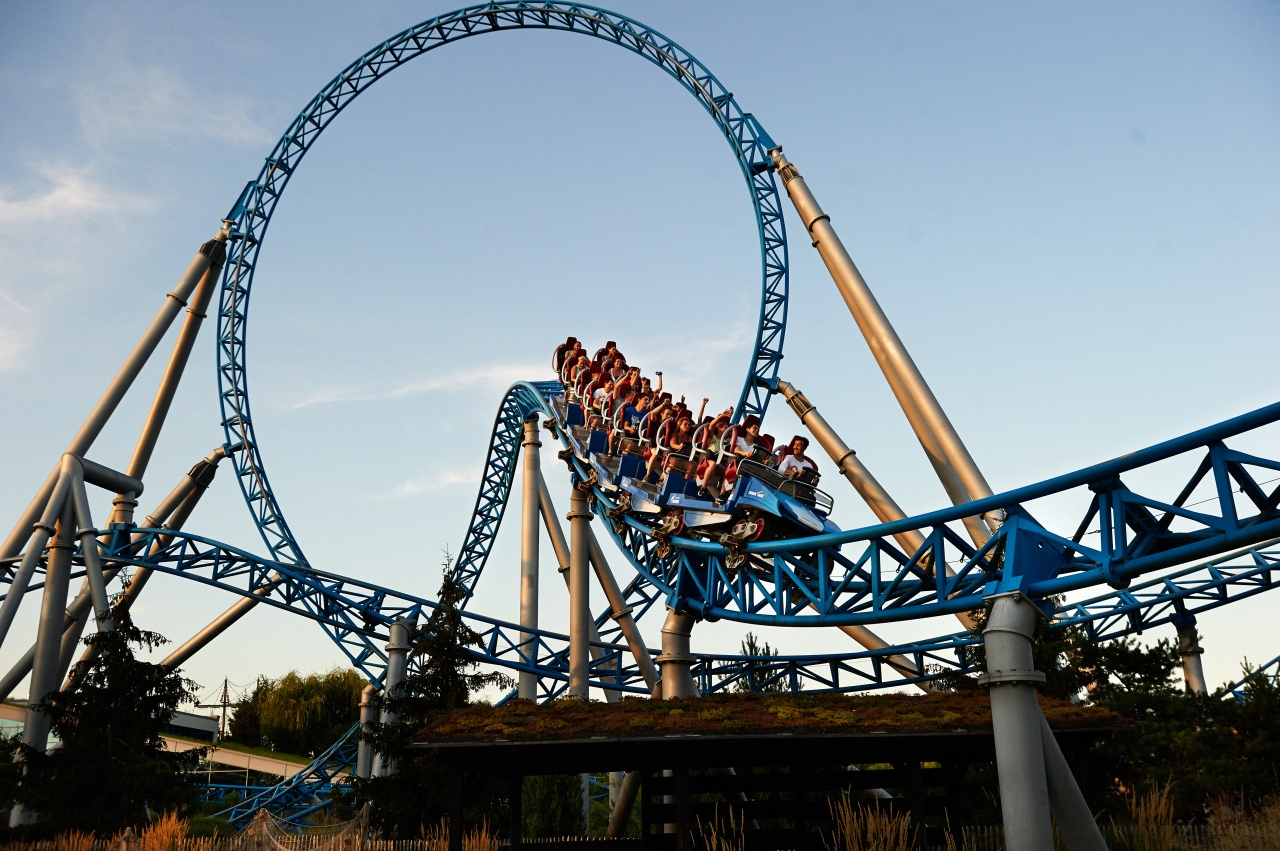
\includegraphics[width=.7\columnwidth]{img/montagnarussa.jpg}
\end{figure}
Immaginiamo una montagna russa ideale, cioè senza attriti di alcun tipo e proponiamone uno schema semplificato.
\end{frame}



\begin{frame}
  \frametitle{Somma costante}
  \begin{figure}
  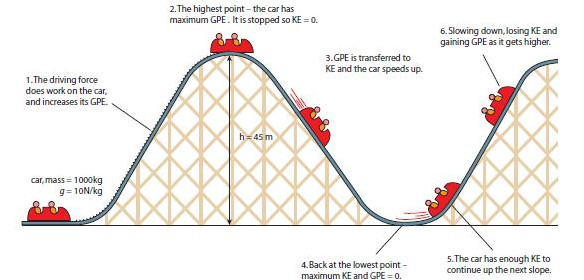
\includegraphics[width=.8\columnwidth]{img/conservazione.jpg}
\end{figure}\pause
Si nota che l'energia cinetica e quella potenziale gravitazionale dei carrelli sono diverse in ogni istante, ma \emph{la loro somma è costante}. Chiamiamo tale somma \alert{energia meccanica del sistema}.
\end{frame}


\begin{frame}
  \frametitle{Conservazione dell'energia}
  Immaginiamo un sistema isolato (su cui non agiscono forze esterne) in cui tutte le forze interne sono conservative.\\~\pause\\  
  Se passiamo da una certa situazione iniziale $ A $ ad una certa situazione finale $ B $, possiamo affermare che \alert<2>{l'energia meccanica totale di un sistema isolato si conserva}:
\begin{center}
\colorbox{blue!30}{$ U_A + K_A = U_B + K_B $}
\end{center}\pause
Questo vale anche per le altre forme di energia possibili:
\begin{block}{Principio di conservazione dell'energia}
  In un sistema isolato l'energia totale si conserva.
\end{block}
\end{frame}


\begin{frame}
\frametitle{Trasferimento di energia}
  Quando una persona salta verso l'alto, essa possiede una certa velocità iniziale, e quindi una certa energia cinetica. Salendo, il lavoro della forza peso \emph<1>{diminuisce l'energia cinetica}, mentre \emph<1>{aumenta l'energia potenziale gravitazionale}.\\~\pause\\In questo e in altri casi, \alert<2>{il lavoro di una forza permette di trasformare una forma di energia in un'altra}.\pause
\begin{block}{Trasferimento di energia}
Il lavoro non è energia, ma è energia in transito (da una forma ad un'altra).
\end{block}
\end{frame}


\begin{frame}
  \frametitle{Esempio 5 (1)}
  \begin{exampleblock}{Conservazione dell'energia durante una caduta}
{\small Un vaso di massa $ 3,00 \, kg $ viene fatto cadere da un'altezza $h = 15,0 \, m $. Una volta raggiunto il suolo, esso rimbalza su una pedana sostenuta da una molla con costante elastica $ 16,0 \, \frac{kN}{m} $.

Calcola:
\begin{itemize}
  \item la velocità con cui il vaso raggiunge la pedana;
  \item di quanto viene compressa la molla.
\end{itemize}}
\end{exampleblock}
  \pause
  L'idea generale del problema è quella di considerare il sistema isolato e impostare di volta in volta l'uguaglianza tra l'energia posseduta nella situazione iniziale e quella posseduta nella situazione finale.
\end{frame}



\begin{frame}
  \frametitle{Esempio 5 (2)}
  Prima di cadere (situazione $ A $) il vaso ha energia potenziale gravitazionale (rispetto al suolo) pari a $ U_{gA} = mgh $ ed energia cinetica nulla. Una volta giunto a terra (situazione $ B $), avrà energia potenziale nulla ed energia cinetica massima.\pause
  \begin{center}
  $ U_{gA} + \cancel{K_A} = \cancel{U_{gB}} + K_B $
  \end{center}\pause
  \begin{center}
    $ \cancel{m}gh = \dfrac{1}{2}\cancel{m}v^2 $
  \end{center}\pause
  \begin{center}
  $ v^2 = 2gh $
  \end{center}\pause
  \begin{center}
  $ v = \sqrt{2gh} = \sqrt{2 \cdot 9,81 \, \frac{m}{s^2}\cdot 15,0 \, m} = 17,2 \, \frac{m}{s}$
  \end{center}
\end{frame}

\begin{frame}
  \frametitle{Esempio 5 (3)}
Quando il vaso colpisce la pedana (situazione $ C $), la sua energia cinetica si converte in energia elastica grazie al lavoro della forza elastica della molla. Vale quindi che:
  \begin{center}
  $ U_{gA} = K_B = U_{eC} $
  \end{center}\pause
  In particolare:
  \begin{center}
    $ \cancel{\dfrac{1}{2}}mv^2 = \cancel{\dfrac{1}{2}}k\Delta x^2 $
  \end{center}\pause
  \begin{center}
  $ \Delta x^2 = \dfrac{mv^2}{k} $
  \end{center}\pause
  \begin{center}
  $ \Delta x = \sqrt{\frac{3,00 \, kg \cdot \left( 17,2 \, \frac{m}{s} \right)^2}{1,60 \times 10^4 \, \frac{N}{m}}} = 0,235 \, m = 23,5 \, cm  $
  \end{center}
\end{frame}




\end{document}
